%\documentclass[xcolor=dvipsnames,12pt]{beamer}

% hide navigation symbols
\beamertemplatenavigationsymbolsempty

% add frame number
% TODO make it simplier
\makeatletter
\setbeamertemplate{footline}
{%
  \leavevmode%
  \hbox{%
  \begin{beamercolorbox}[wd=.92\paperwidth,ht=2.25ex,dp=1ex,center]{title in head/foot}%
  \end{beamercolorbox}%
  \begin{beamercolorbox}[wd=.08\paperwidth,ht=2.25ex,dp=1ex,leftskip=0cm plus1fill,rightskip=.015\paperwidth]{page number in head/foot}%
    \usebeamerfont{page number in head/foot}
    \insertframenumber{}
  \end{beamercolorbox}}%
  \vskip5pt%
}
\makeatother


% simple section page
\defbeamertemplate{section page}{simple}[1][]{
  \begin{centering}
    {\usebeamerfont{section name}\usebeamercolor[fg]{section name}#1}
    \vskip1em\par
    \begin{beamercolorbox}[sep=12pt,center]{part title}
      \usebeamerfont{section title}\insertsection\par
    \end{beamercolorbox}
  \end{centering}
}
\setbeamertemplate{section page}[simple]
\AtBeginSection{
  \frame[plain,c]{\sectionpage}
}

% mimic plain frame from metropolis theme
\newcommand{\plain}[2][]{%
  \begingroup
    \begin{frame}[plain,c]{#1}
      \begin{center}
        \usebeamercolor[fg]{frametitle}
        \bfseries\Large #2
      \end{center}
    \end{frame}
  \endgroup
}

% code colors
\colorlet{codeString}{Green}
\colorlet{codeKeyword}{RedOrange}
\colorlet{codeComment}{Gray}


% workaround for problem with white text if notes are enabled
% http://tex.stackexchange.com/questions/232168/normal-text-is-invisible-when-using-beamer-with-notes-and-xelatex
\def\pgfsysdriver{pgfsys-dvipdfm.def}

\documentclass[xcolor=dvipsnames]{beamer}

\usetheme{metropolis}
\setbeamercolor{normal text}{bg=white} % white background instead of black!2

% Fira Mono looks ugly, especially "0" & "&"
\setmonofont{Inconsolata}
% workaround for "Package polyglossia Error: The current roman font does not contain the Cyrillic script!"
\newfontfamily\cyrillicfonttt{Inconsolata}

% code colors from metropolis
\colorlet{codeString}{mLightGreen}
\colorlet{codeKeyword}{mLightBrown}
\colorlet{codeComment}{Gray}


\usepackage{ifxetex}

\ifxetex
  \usepackage{polyglossia}
  \setmainlanguage{russian}
  \setotherlanguage{english}

  % workaround for "Package polyglossia Error: The current roman font does not contain the Cyrillic script!"
  \newfontfamily\cyrillicfonttt{Fira Mono}
\else
  \usepackage[T2A]{fontenc}
  \usepackage[utf8]{inputenc}
  \usepackage[english,russian]{babel}

  % workaround for "Package hyperref Warning: Glyph not defined in PD1 encoding"
  \hypersetup{unicode=true}
\fi

\newcommand{\eng}[1]{%
  \ifxetex%
    {\textenglish{#1}}%
  \else%
    {\foreignlanguage{english}{#1}}%
  \fi%
}

\usepackage{pgfpages}

% minimal - it is like plain, but with background color
\defbeamertemplate{note page}{minimal}{%
  \nointerlineskip%
  \insertvrule{\paperheight}{note page.bg}%
  \vskip-\paperheight%
  \insertnote%
}

%\setbeameroption{show notes on second screen}
\setbeamertemplate{note page}[minimal]
\setbeamercolor{note page}{bg=black!5}

\newcommand{\notep}[1]{\note{#1\par}}


\usepackage{listings}
\usepackage{lstautogobble}
\lstset{
  xleftmargin=0.03\textwidth,
  aboveskip=0.75\medskipamount,
  belowskip=0.5\medskipamount,
  %
  basicstyle=\ttfamily\small,
  keywordstyle=\color{codeKeyword},
  stringstyle=\color{codeString},
  commentstyle=\color{codeComment},
  %
  literate={-}{-}1, % render dash as dash
  showstringspaces=false,
  %
  autogobble
}

\lstdefinelanguage{myC}[]{C}{
  morekeywords={size_t}
}

\lstdefinestyle{inlineC}{%
  basicstyle=\ttfamily\normalsize,
  language=myC
}

\lstnewenvironment{clisting}[1][]{\lstset{language=myC,#1}}{}

\newcommand{\comment}[1]{\color{codeComment}#1}

% Workaround for unconditional parskip after lstlisting environment
% See: http://tex.stackexchange.com/questions/40863/parskip-inserts-extra-space-after-floats-and-listings
\newcommand{\revertListingParskip}{%
  \vspace*{-\parskip}%
}



\hypersetup{pdfauthor={Владимир Владимирович Парфиненко}}
\title{Основы программирования}
\subtitle{Лекция № 2, 1 марта 2018 г.}
\date{}
\institute{
  \vspace{1em}
  \centering
  \parbox{0.9\textwidth}{
    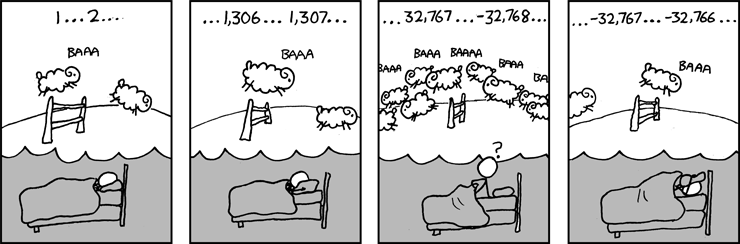
\includegraphics[width=\linewidth]{xkcd_cant_sleep}
    \par
    \raggedleft\tiny\url{http://xkcd.com/571}
  }
}


\begin{document}

% it can be done only after begin{document} because of "@"
\lstMakeShortInline[style=inlineC]@

\begin{frame}[plain]
  \titlepage
\end{frame}

% This frames uses @ symbol
\lstDeleteShortInline@
\begin{frame}{Знакомство}

  Я~--- Владимир Владимирович Парфиненко,

  \begin{itemize}
    \item бакалавр физики (ФФ), магистр математики (ММФ),
    \item профессиональный программист (Excelsior),
    \item регулярно чему-то учу (ФФ, АФТИ, ЛШ ФМШ).
  \end{itemize}


  Контакт:
  \href{mailto:vladimir.parfinenko@gmail.com}{vladimir.parfinenko@gmail.com}

\end{frame}
\lstMakeShortInline[style=inlineC]@

\section{Целочисленные типы данных}
\notep{
  Заметим, что с помощью двух ламп можно представить числа от 0 до 3.
}

\begin{frame}{Двоичная система счисления}

  Самый простой метод записи чисел, использующий только две цифры: 0 и 1.
  \notep{Компьютеру легко работать с такими числами.}

  С помощью $n$ \emph{позиций} можно записать $2^n$ чисел.
  \notep{Индекс $x_{10}$ будем опускать.}
  \begin{align*}
    \bin{000} &= 0, &\qquad \bin{100} &= 4, \\
    \bin{001} &= 1, &\qquad \bin{101} &= 5, \\
    \bin{010} &= 2, &\qquad \bin{110} &= 6, \\
    \bin{011} &= 3, &\qquad \bin{111} &= 7.
  \end{align*}

  \notep{Правила перевода из двоичной в десятичную и обратно выходит за рамки
    данной лекции.}
\end{frame}

\begin{frame}[fragile]{Числа в памяти компьютера}

  1 \emph{байт} состоит из 8 \emph{бит} и может кодировать $2^8 = 256$
  различных чисел.
  \notep{Байт - минимальная ячейка памяти, которую компьютер может
  читать/писать.}

  Например, число 337 кодируется минимум 2 байтами:
  \[
    \underbrace{\pcnum{00000001}}_{\text{биты } 15 \ldots 8}
    \underbrace{\pcnum{01010001}}_{\text{биты } 7 \ldots 0}
  \]

  \begin{itemize}
    \item 1 байт (8 бит) кодирует $\num{256}$ чисел,
    \item 2 байта (16 бит) кодируют $\num{65536}$ чисел,
    \item 4 байта (32 бита) кодируют $\num{4294967296}$ чисел,
    \item 8 байт (64 бита) кодируют $\num{18446744073709551616}$ чисел.
      \notep{$\num{18e18}$ = восемнадцать квинтиллионов.}
  \end{itemize}

\end{frame}

\begin{frame}[fragile]{Целочисленные типы в \eng{C}}

  \notep{Эти значения могут варьироваться в зависимости от платформы и
    компилятора.}

  \begin{table}
    \begin{tabular}{cccc}
      \hline
      Тип         & Размер, бит & Минимум & Максимум  \\
      \hline

      \pause
      @unsigned char@      & 8  & 0       & $\num{255}$ \\
      @unsigned short@     & 16 & 0       & $\num{65535}$ \\
      @unsigned int@       & 32 & 0       & $\num{4294967295}$ \\
      @unsigned long long@ & 64 & 0       & $\num{18.4e18}$ \\
      \hline

      \pause
      @signed char@        & 8  & $\num{-128}$        & $\num{127}$ \\
      \notep{Знаковость char не стандартизирована.}
      @short@              & 16 & $\num{-32768}$      & $\num{32767}$ \\
      @int@                & 32 & $\num{-2147483648}$ & $\num{2147483647}$ \\
      @long long@          & 64 & $\num{-9.2e18}$     & $\num{9.2e18}$ \\
      \hline

      \notep{
        Знак хранится в тех же самых 8/16/... битах.
        Детали представления отрицательных чисел выходят за рамки данной
        лекции.
      }

    \end{tabular}
  \end{table}

\end{frame}

\begin{frame}{Сложение целых чисел с переполнением}

  Рассмотрим сложение двух 8-битных беззнаковых чисел
  \[250 + 9 = \pause \bin{1111\,1010} + \bin{0000\,1001} = \ldots\]
  \pause
  \[
    \begin{array}{r}
    +
      \begin{array}{r}
        \pcnum{1111\,1010} \\
        \pcnum{0000\,1001} \\
      \end{array} \\
      \hline
      \pause
      \begin{array}{r}
        \pcnum{1}\underbrace{\pcnum{0000\,0011}}_{8 \text{ бит}}
      \end{array}
    \end{array}
  \]

  \pause
  С точки зрения компьютера: $250 + 9 = \bin{0000\,0011} = 3$.

  \notep{
    То есть компьютер выполняет сложение и вычитание по модулю,
    соответствующему размеру числа, т.е. отбрасывает старшую часть.
  }

\end{frame}

\begin{frame}{Виды переполнения целых чисел}

  \begin{columns}[onlytextwidth,c]
    \begin{column}{0.5\textwidth}
      \begin{block}{Беззнаковые 8-битные:}
        \begin{itemize}
          \item $255 + 1 = 0$,
          \item $0 - 1 = 255$.
        \end{itemize}
      \end{block}
      \notep{Переполнение беззнаковых чисел в \eng{C} стандартизовано.}
    \end{column}

    \pause

    \begin{column}{0.5\textwidth}
      \begin{block}{Знаковые 8-битные:}
        \begin{itemize}
          \item $127 + 1 = -128$,
          \item $-128 - 1 = 127$.
        \end{itemize}
      \end{block}
      \notep{Переполнение знаковых чисел в \eng{C}~--- неопределенное поведение.}
    \end{column}

  \end{columns}

  \notep{Про переполнение надо знать, но лучше на него не полагаться.}

\end{frame}

\begin{frame}{\eng{Epic Fails}}

  \begin{itemize}
    \pause
    \item 13 июня 2009 г.~--- \eng{Twitter}: порядковый номер твитов
      переполнил 32-битное знаковое целое.
    \pause
    \item 22 сентября 2009 г.~--- \eng{Twitter}: порядковый номер твитов
      переполнил 32-битное беззнаковое целое.
    \pause
    \item 9 февраля 2013 г.~--- \eng{OpenStreetMap}: порядковый номер точек на
      карте переполнил 32-битное знаковое целое.
    \pause
    \item 1 декабря 2014 г.~--- \eng{YouTube}: количество просмотров
      \href{https://www.youtube.com/watch?v=9bZkp7q19f0}{одного видео}
      переполнило 32-битное знаковое целое.
    \pause
    \item 20 января 2017 г.~--- \eng{Code.org}: идентификатор студенческих
      работ переполнил 32-битное беззнаковое целое.
  \end{itemize}

  \notep{В абсолютном большинстве случаев хватит 32-битных чисел.}

\end{frame}


\section{Вещественные типы данных}

\begin{frame}{Числа с плавающей точкой}

  \notep{Трудности перевода: в России разделителем служит запятая.}

  {\Large \[ x = m \cdot b^e, \] }
  где:
  \begin{itemize}
    \item $m$~--- \emph{мантисса} (значащая часть),
    \item $b$~--- \emph{основание степени} (обычно 2 или 10),
    \item $e$~--- \emph{экспонента} (порядок).
  \end{itemize}
  \notep{Очень привычная для физиков форма записи вещественный чисел.}

\end{frame}

\begin{frame}[fragile]{Числа с плавающей точкой в \eng{C}}

  \begin{table}
    \begin{tabular}{cccc}
      \hline
      Тип      & Мин. абс. значение & Макс. абс. значение & Точность, дес. знаков \\
      \hline
      @float@  & $\num{1.18e-38}$   & $\num{3.40e38}$     & $\approx 7$ \\
      @double@ & $\num{2.23e-308}$  & $\num{1.80e308}$    & $\approx 16$ \\
      \hline
    \end{tabular}
  \end{table}
  \notep{
    Точность binary32: $\log_{10}(2^{23}+1) \approx \num{7.225}$,\\
    точность binary64: $\log_{10}(2^{52}+1) \approx \num{15.955}$.
  }
  \notep{Мин. и макс. значения даны для нормализованных чисел.}
  \notep{Проще всегда использовать double.}



\end{frame}

\begin{frame}{Особенные числа}

  \begin{block}{Числа $\pm 0$, $\pm \infty$}
    \reduceBlockEqSpacing
    \begin{gather*}
      \log(0) = -\infty, \\
      1 / (+0) = +\infty, \\
      1 / (-0) = -\infty.
    \end{gather*}
  \end{block}

  \pause

  \newcommand{\NaN}{NaN}

  \begin{block}{Не-числа (\eng{NaN, Not a Number}):}
    \reduceBlockEqSpacing
    \begin{gather*}
      \NaN = \sqrt{-1}, 0 / 0, 0 \cdot \infty, \infty / \infty, \infty - \infty, \\
    \end{gather*}
  \end{block}

  \let\NaN\undefined

  \notep{Есть еще денормализованные числа, но это выходит за рамки данной
    лекции.}

\end{frame}

\begin{frame}{Проблемы с точностью}

  \begin{itemize}[<+->]
    \item Округление: $\tg(\pi) \neq 0, \tg(\pi/2) \neq \infty$.
    \item Накопление ошибок:
      $a + (b + c) \neq (a + b) + c$.
    \item Потеря точности:
      $a - b$, если $a \approx b$.
      \notep{$\frac{f(a)-f(b)}{a-b}$~--- в числителе значащими становятся младшие,
        неточные разряды.}
    \item Потеря точности:
      $a + b$, если $a \gg b$ или $a \ll b$.
    \item Сравнение чисел.
  \end{itemize}

  \notep{Вещественные числа нужно сравнивать приблизительно. Подробности
    выходят за рамки этой лекции.}

\end{frame}


\section{Массивы}
\notep{
  Мотивация: для задания квадратного уравнения нужно 3 переменные: a, b, c.
  А что делать с уравнением 10-ой степени?
  Правильно, нужен массив!
}

\begin{frame}[fragile]{Объявление массива}

  Массив~--- упорядоченный набор элементов одного типа.

  \pause
  Объявление массива @arr@, состоящего из @N@ элементов произвольного
  типа~@T@:
  \begin{clisting}
    T arr[N];
  \end{clisting}
  \revertListingParskip
  где @N@~--- константа времени компиляции.
  \notep{Без инициализации массив, объявленный в функции, содержит мусор.}

  \pause
  Пример объявления и инициализации массива:
  \begin{clisting}
    int xs[4];            // {?, ?, ?, ?}
    int ys[]  = {20, 10}; // {20, 10}
    int zs[4] = {20, 10}; // {20, 10, 0, 0}
  \end{clisting}
  \notep{Элементы, для которых нет явно заданного значения, инициализируются
    нулями.}
  \notep{Размер массива может быть вычислен автоматически, что может быть
    довольно удобным.}

\end{frame}

\tikzset{array matrix/.style={matrix of nodes, nodes in empty cells,
  column sep=-\pgflinewidth, row sep=-\pgflinewidth}}
\tikzset{array node/.style={draw, anchor=center, minimum height=9mm, minimum width=9mm}}
\tikzset{array index node/.style={align=center, anchor=center, text width=6mm}}

\begin{frame}[fragile]{Доступ к элементам массива}

  @T arr[N]@:
  \begin{center}
  \begin{tikzpicture}
    \matrix (m) [array matrix,
      row 1/.style={nodes={array node}},
      row 2/.style={nodes={array index node}}
    ]{
          &     & &        & &       \\
      @0@ & @1@ & & \ldots & & @N-1@ \\
    };
  \end{tikzpicture}
  \end{center}
  \notep{Индексы в массиве от 0 до N-1.}

  \pause
  Чтение элемента из массива по индексу @i@:
  \begin{clisting}
    T value = arr[i];
  \end{clisting}

  Запись элемента в массив по индексу @i@:
  \begin{clisting}
    arr[i] = new_value;
  \end{clisting}

  \notep{Доступ по недопустимому индексу (-1, N, 2*N)~--- неопределенное
    поведение.}

\end{frame}


\section{Указатели}

\tikzset{
  byte lines/.style={black!30},
  block byte lines/.style={black!40},
  mem block/.style={fill=black!10},
}

\newcommand\memtop{1}
\newcommand\membottom{0}

\newcommand{\memline}[2]{
  \def\left{#1-0.45}
  \def\right{#2+0.45}

  \draw[byte lines] (\left,\membottom) grid (\right,\memtop);

  \foreach \y in {\membottom, \memtop}
    \draw (\left,\y) -- (\right,\y);

  \foreach \x in {\left, \right}
    \draw [decorate,decoration={snake,amplitude=0.3mm,segment length=3mm}]
      (\x,\membottom) -- (\x,\memtop);
}

\newcommand{\memblock}[3]{
  \def\left{#1}
  \def\right{#2}
  \def\blockname{#3}

  \draw [mem block,draw=none] (\left,\membottom) rectangle (\right,\memtop);
  \draw [block byte lines] (\left,\membottom) grid (\right,\memtop);
  \draw [mem block,fill=none] (\left,\membottom) rectangle (\right,\memtop)
    node [pos=0.5] (block \blockname) {};
}

\newcommand{\memaddr}[2]{
  \def\x{#1+0.5}
  \def\y{\membottom-0.5}
  \draw [-latex,shorten <=6pt] (\x,\y)
    node [fill=white,inner sep=0,outer sep=0] {\ttfamily\small #2} -- (\x,\membottom);
}

\newcommand{\memlabel}[3]{
  %\draw [decorate,decoration={brace, raise=0.7mm}] (#1,\memtop) -- (#2,\memtop)
  %  node [midway,yshift=4mm] {\ttfamily #3};
  \path (#1,\memtop) -- (#2,\memtop)
    node [midway,yshift=3mm,text height=1.5ex] {\ttfamily #3};
}

\newcommand{\memblockwithaddr}[5]{
  \memblock{#1}{#2}{#3}
  \memaddr{#1}{#4}
  \memaddr{#2-1}{#5}
}

\newcommand{\memblockwithaddrandlabel}[6]{
  \memblockwithaddr{#1}{#2}{#3}{#4}{#5}
  \memlabel{#1}{#2}{#6}
}

\newcommand{\memblockwithoneaddr}[4]{
  \memblock{#1}{#2}{#3}
  \memaddr{#1}{#4}
}

\newcommand{\memblockwithoneaddrandlabel}[5]{
  \memblockwithoneaddr{#1}{#2}{#3}{#4}
  \memlabel{#1}{#2}{#5}
}

\begin{frame}[fragile]{Указатель как адрес}

  \begin{center}
  \begin{visibleenv}<2->
  \begin{tikzpicture}[
      scale=0.8,
  ]

    \memline{1}{7}
    \memblock{2}{6}{x}
    \node [mem block] at (block x) {518};

    \memline{8}{14}
    \memblock{9}{13}{y}
    \node<-7> [mem block] at (block y) {320};
    \node<8-> [mem block] at (block y) {999};

    \begin{visibleenv}<3->
      \memaddr{2}{0x20}
      \memaddr{5}{0x23}

      \memaddr{9}{0x40}
      \memaddr{12}{0x43}
    \end{visibleenv}
  \end{tikzpicture}
  \end{visibleenv}
  \end{center}

  \begin{columns}[onlytextwidth,T]
    \begin{column}{0.25\textwidth}
      \begin{clisting}[escapechar=\!]
        int x = 518;
        int y = 320;
      \end{clisting}
    \end{column}

    \begin{column}{0.75\textwidth}<4->
      \begin{clisting}[escapechar=\!]
        int* ptr;
        !\onslide<5->!// !\comment\& - взятие адреса!
        // !\comment* - разыменование указателя!
        ptr = &x;
        printf("%p %d\n", ptr, *ptr); // 0x20 518
        !\onslide<6->!ptr = &y;
        printf("%p %d\n", ptr, *ptr); // 0x40 320
        !\onslide<7->!*ptr = 999;
        !\onslide<9->!printf("%d %d\n", x, y); // 518 999
      \end{clisting}
    \end{column}

  \end{columns}

  \notep{Адресом блока памяти считается номер его самого младшего байта.}
  \notep{int*~--- указатель на int, т.е. адрес памяти, где лежит int.}
  \notep{Заметьте, y поменяло свое значение, хотя прямых записей в него не было.}
  \notep{0x*** - это шестнадцатеричная запись числа, именно в таком виде
    принято записывать значения адресов. И именно в таком виде их выводит
    printf с модификатором \%p.}

\end{frame}

\begin{frame}[fragile]{Массивы и указатели}

  \begin{center}
  \begin{visibleenv}<2->
  \begin{tikzpicture}[
      scale=0.8,
  ]
    \memline{1}{9}
    \memblockwithoneaddrandlabel{2}{4}{a0}%
      {0x20}%
      {a[0]}
    \memblockwithoneaddrandlabel{4}{6}{a1}%
      {0x22}%
      {a[1]}
    \memblockwithoneaddrandlabel{6}{8}{a2}%
      {0x24}%
      {a[2]}

    \node [mem block] at (block a0) {10};
    \node<-5> [mem block] at (block a1) {20};
    \node<6-> [mem block] at (block a1) {200};
    \node<-7> [mem block] at (block a2) {30};
    \node<8-> [mem block] at (block a2) {230};

  \end{tikzpicture}
  \end{visibleenv}
  \end{center}

  \begin{columns}[onlytextwidth,T]<-13>
    \begin{column}{0.5\textwidth}
      \begin{clisting}[escapechar=\!]
        short a[3] = {10, 20, 30};

        !\onslide<3->!short* p = !\temporal<12>{!\&(a[0])!}{!\&(*(a))!}{!a!}!; // 0x20
        !\onslide<4->!short* p1 = p + 1;  // 0x22
        short* p2 = p + 2;  // 0x24
      \end{clisting}
    \end{column}

    \begin{column}{0.45\textwidth}
      \begin{clisting}[escapechar=\!]
        !\onslide<5->!!\temporal<9-10>{!*p1!}{!*(p+1)!}{!p[1]!}! = 200;
        !\onslide<7->!!\temporal<9-10>{!*p2!}{!*(p+2)!}{!p[2]!}! = !\temporal<9-10>{!*p1!}{!*(p+1)!}{!p[1]!}! + !\temporal<9-10>{!*p2!}{!*(p+2)!}{!p[2]!}!;
        !\onslide<10->!// *(x + y) == x[y]
      \end{clisting}
    \end{column}

  \end{columns}

  \notep{Массив хранится как непрерывный блок памяти, элементы располагаются
    последовательно.}
  \notep{При прибавлении значения n к указателю, его значение увеличивается на
    (n * размер типа данных под указателем).}
  \notep{Массивная переменная~--- всего лишь указатель на начало массива.}

\end{frame}


\plain{Остальное не влезло в пару… Про запас нужно взять несколько слайдов со
следующей лекции.}


\plain{Конец второй лекции}


\begin{backup}


\section{Секретные слайды}


\begin{frame}[fragile]{Загадка: модуль числа неотрицательный?}

  \begin{block}{Вычисление модуля введенного числа:}
    \begin{lstlisting}[language=C]
    int x;
    printf("Enter number: ");
    scanf("%d", &x);
    if (x < 0) {
        x = -x;
    }
    printf("Absolute value = %d\n", x);
    \end{lstlisting}
  \end{block}

  \begin{block}{Исполнение:}
    \begin{onlyenv}<1>\begin{lstlisting}
    Enter number: -37
    Absolute value = 37
    \end{lstlisting}\end{onlyenv}
    \begin{onlyenv}<2>\begin{lstlisting}
    Enter number: -2147483648
    Absolute value = -2147483648
    \end{lstlisting}\end{onlyenv}
    \notep{Все из-за переполнения.}
  \end{block}

\end{frame}


\begin{frame}[fragile]{Неправильное сравнение чисел}

  \begin{columns}[onlytextwidth,c]
    \begin{column}{0.6\textwidth}
      \begin{lstlisting}[language=C,escapechar=\!]
float x = 0.1f;
float y1 = x * x;
float y2 = 0.01f;

y1 == y2; !\visible<2->{\color{codeComment}// => 0}!
      \end{lstlisting}
    \end{column}

    \begin{column}<3->{0.4\textwidth}
      
\includegraphics[width=\linewidth]{meme_why}
    \end{column}

  \end{columns}

\end{frame}

\begin{frame}[fragile]{Причина неправильного сравнения чисел}

  \begin{lstlisting}[language=C,escapechar=\!]
float x = 0.1f; // 0.100000001490
float y1 = x * x;
// 0.010000000708 =
//    0 01111000 0100011110101110000101!\alert{1}!
float y2 = 0.01f;
// 0.009999999776 =
//    0 01111000 0100011110101110000101!\alert{0}!

y1 == y2; // => 0
  \end{lstlisting}
  \notep{Отличие в одном бите мантиссы в бинарном представлении.}

\end{frame}

\begin{frame}[fragile]{Правильное сравнение чисел}

  Идея:
  \begin{lstlisting}[language=C]
fabs(y1 - y2) < 0.00001f; // => 1
  \end{lstlisting}

  \pause

  Но нужно так же учесть:
  \begin{itemize}
    \item очень большие и очень маленькие числа,
    \item бесконечности,
    \item \ldots
  \end{itemize}

  Реализация: \href{%
    https://github.com/cypok/floats-comparison%
  }{%
    github.com/cypok/floats-comparison
  }

\end{frame}


\end{backup}


\end{document}
